\documentclass[conference]{IEEEtran}

\usepackage{cite}
\usepackage{amsmath,amssymb,amsfonts}
\usepackage{algorithmic}
\usepackage{graphicx}
\usepackage{textcomp}
\usepackage{xcolor}
\usepackage{hyperref}
\usepackage{cleveref}
\usepackage{commath}
\usepackage{optidef}
\setlength{\tabcolsep}{10pt}
\renewcommand{\arraystretch}{1.45}

\def\BibTeX{{\rm B\kern-.05em{\sc i\kern-.025em b}\kern-.08em
    T\kern-.1667em\lower.7ex\hbox{E}\kern-.125emX}}
\begin{document}

\title{Performance Analysis of STAR-RIS Enhanced CoMP-NOMA Multi-Cell Networks}

\author{
\IEEEauthorblockN{
	Muhammad Umer\IEEEauthorrefmark{1},
	Muhammad Ahmed Mohsin\IEEEauthorrefmark{1},
	Syed Ali Hassan\IEEEauthorrefmark{1},
	Haejoon Jung\IEEEauthorrefmark{2},
	and Haris Pervaiz\IEEEauthorrefmark{3}}
\IEEEauthorblockA{\IEEEauthorrefmark{1}School of Electrical Engineering and Computer Science (SEECS), NUST, Pakistan}
\IEEEauthorblockA{\IEEEauthorrefmark{2}Department of Electronics and Information Convergence Engineering, Kyung Hee University, Republic of Korea}
\IEEEauthorblockA{\IEEEauthorrefmark{3}School of Computing and 
Communications, Lancaster University, UK}
\IEEEauthorblockA{Email: \{mumer.bee20seecs, mmohsin.bee20seecs, ali.hassan\}@seecs.edu.pk, \\haejoonjung@khu.ac.kr, h.b.pervaiz@lancaster.ac.uk}
}
\maketitle

\begin{abstract}
In this paper, we present a novel approach to enhance data rates in a multi-cell network through a pertinent combination of simultaneously transmitting and reflecting reconfigurable intelligent surfaces (STAR-RISs), non-orthogonal multiple access (NOMA), and coordinated multi-point transmission (CoMP). Through the strategic deployment of STAR-RISs, data rates for cell-edge users are significantly improved. The system's overall performance is further optimized by employing exhaustive computation techniques. Additionally, this paper investigates the impact of both the presence and absence of the CoMP technique on outage conditions and data rates. These findings offer valuable insights for the future design and optimization of wireless communication systems.
\end{abstract}

\begin{IEEEkeywords}
	NOMA, CoMP, STAR-RIS
\end{IEEEkeywords}

\section{Introduction}
Reconfigurable intelligent surfaces (RISs) offer a promising solution for enhancing spectral efficiency (SE) and coverage in sixth-generation (6G) wireless networks~\cite{wu2019towards, di2020smart}. They are essentially a 2-D metasurface equipped with low-cost, eco-friendly passive elements. Being passive in nature, these devices can enhance signal coverage by adjusting both phase and amplitude so that the signals are combined constructively at the desired receiver. Their passive behavior promotes green internet in digital ecosystems, providing higher data rates and spectral efficiency while being cost-effective. RIS only passively recycles signals that are already part of the wireless network. Despite its advantage of improving the data rates and signal coverage, these surfaces impose a problem called the half-space problem, which requires that the impinging signal and the user must be located on the same side of RIS, introducing additional constraints to the system, as in~\cite{hou2021joint}.

To overcome this limitation, recent research in developing metasurfaces and advanced fabrication technologies led to a novel idea of simultaneously transmitting and reflecting RIS (STAR-RIS), which divides its elements so that some take part in reflection and the rest in transmission. STAR-RIS can enhance the non-line-of-sight (NLoS) coverage of the impinging signal by providing a virtual line-of-sight path by establishing links to both surfaces, which can solve the half-space problem.

The quest for improved performance in cellular networks has prompted the deployment of numerous low-power, cost-effective, and compact (BSs). However, this proliferation has given rise to a formidable cross-tier inter-cell interference (ICI) obstacle, which hinders further advancements. Furthermore, the substantial power consumption resulting from the dense BS deployment presents a pressing challenge.

Coordinated multi-point (CoMP) techniques have emerged as a promising solution to address these issues. Through high-speed fronthaul links and the sharing of channel state information (CSI) among BSs, CoMP networks allow for the mitigation of ICI and the consequent enhancement of overall network performance. CoMP was introduced in the Long Term Evolution Advanced (LTE-A) Release 11 by the third generation partnership project (3GPP), which become a crucial component for 5G communications. However, coordination among all the BSs is challenging in practice due to inaccurate CSI, additional synchronization across cells, and additional signal processing. Making clusters for CoMP wireless systems is also an optimization problem for future wireless networks.

On the other hand, multiple access techniques have been established to increase the spectral efficiency of wireless systems, and non-orthogonal multiple access (NOMA) is one of them. The power-domain NOMA superposes multiple users in the power domain. However, the downlink signal could be transmitted based on any other baseline in the LTE system. 

In this paper, we consider a STAR-RIS-enhanced CoMP-NOMA network and present a detailed analysis of the achievable rates of cellular users. The main contributions of this paper can be summarized as follows.
\begin{itemize}
    \item  A novel model for the joint utilization of
    STAR-RISs and CoMP-NOMA to enhance the system performance in a multi-cell network. By strategically deploying STAR-RISs, we are able to improve the network coverage and outage conditions of the cell-edge user.
    \item Investigating the impact of CoMP and non-CoMP systems on diverse performance metrics, we demonstrate the superiority of strategically placed and optimized STAR-RISs over conventional systems.
    \item Investigating the impact of pertinently assigning STAR-RIS elements to BSs based on the channel conditions and optimizing amplitude adjustments for transmission and reflection regions on the achievable network sum-rate.

\end{itemize}

\section{System Model}
\subsection{System Layout}
As shown in Fig. \ref{fig:system}, we consider a narrow-band two-cell CoMP-NOMA downlink communication system operating over frequency-flat channels with a STAR-RIS comprising $K$ elements, which are strategically positioned at the intersection of the cells.
% The dynamic elements of the STAR-RIS can be assigned to simultaneously transmit and reflect the signal from either of the two BSs, but not both.
Let the index sets be defined as $\mathcal{I} = \{1, 2\}$ for the two BSs, $\mathcal{C} = \{1, 2,\dots, C\}$ for the cell-center users, and $\mathcal{F} = \{1, 2,\dots, F\}$ for the cell-edge users, where $C$, and $F$ represent the cardinality of $\mathcal{C}$, and $\mathcal{F}$, respectively. Additionally, let $\mathcal{U} = \{\mathcal{M}\cup\,\mathcal{N}\,\cup\,\mathcal{F}\}$ be the set of all users in the system. For simplicity, we only focus on the typical scenario, where each BS is equipped with a single antenna, establishing communication links with one single-antenna cell-center user and one single-antenna cell-edge user. Thus, in this context, we have $M=1$, $N=1$, and $F=1$. In addition, $\forall c \in \mathcal{C}$, $\forall f \in \mathcal{F}$, U$_c$ is placed in the reflection region $\mathbf{\Theta_r}$, while U$_f$ is placed in the transmission region $\mathbf{\Theta_t}$ of the STAR-RIS.

\begin{figure}[t]
    \centerline{
        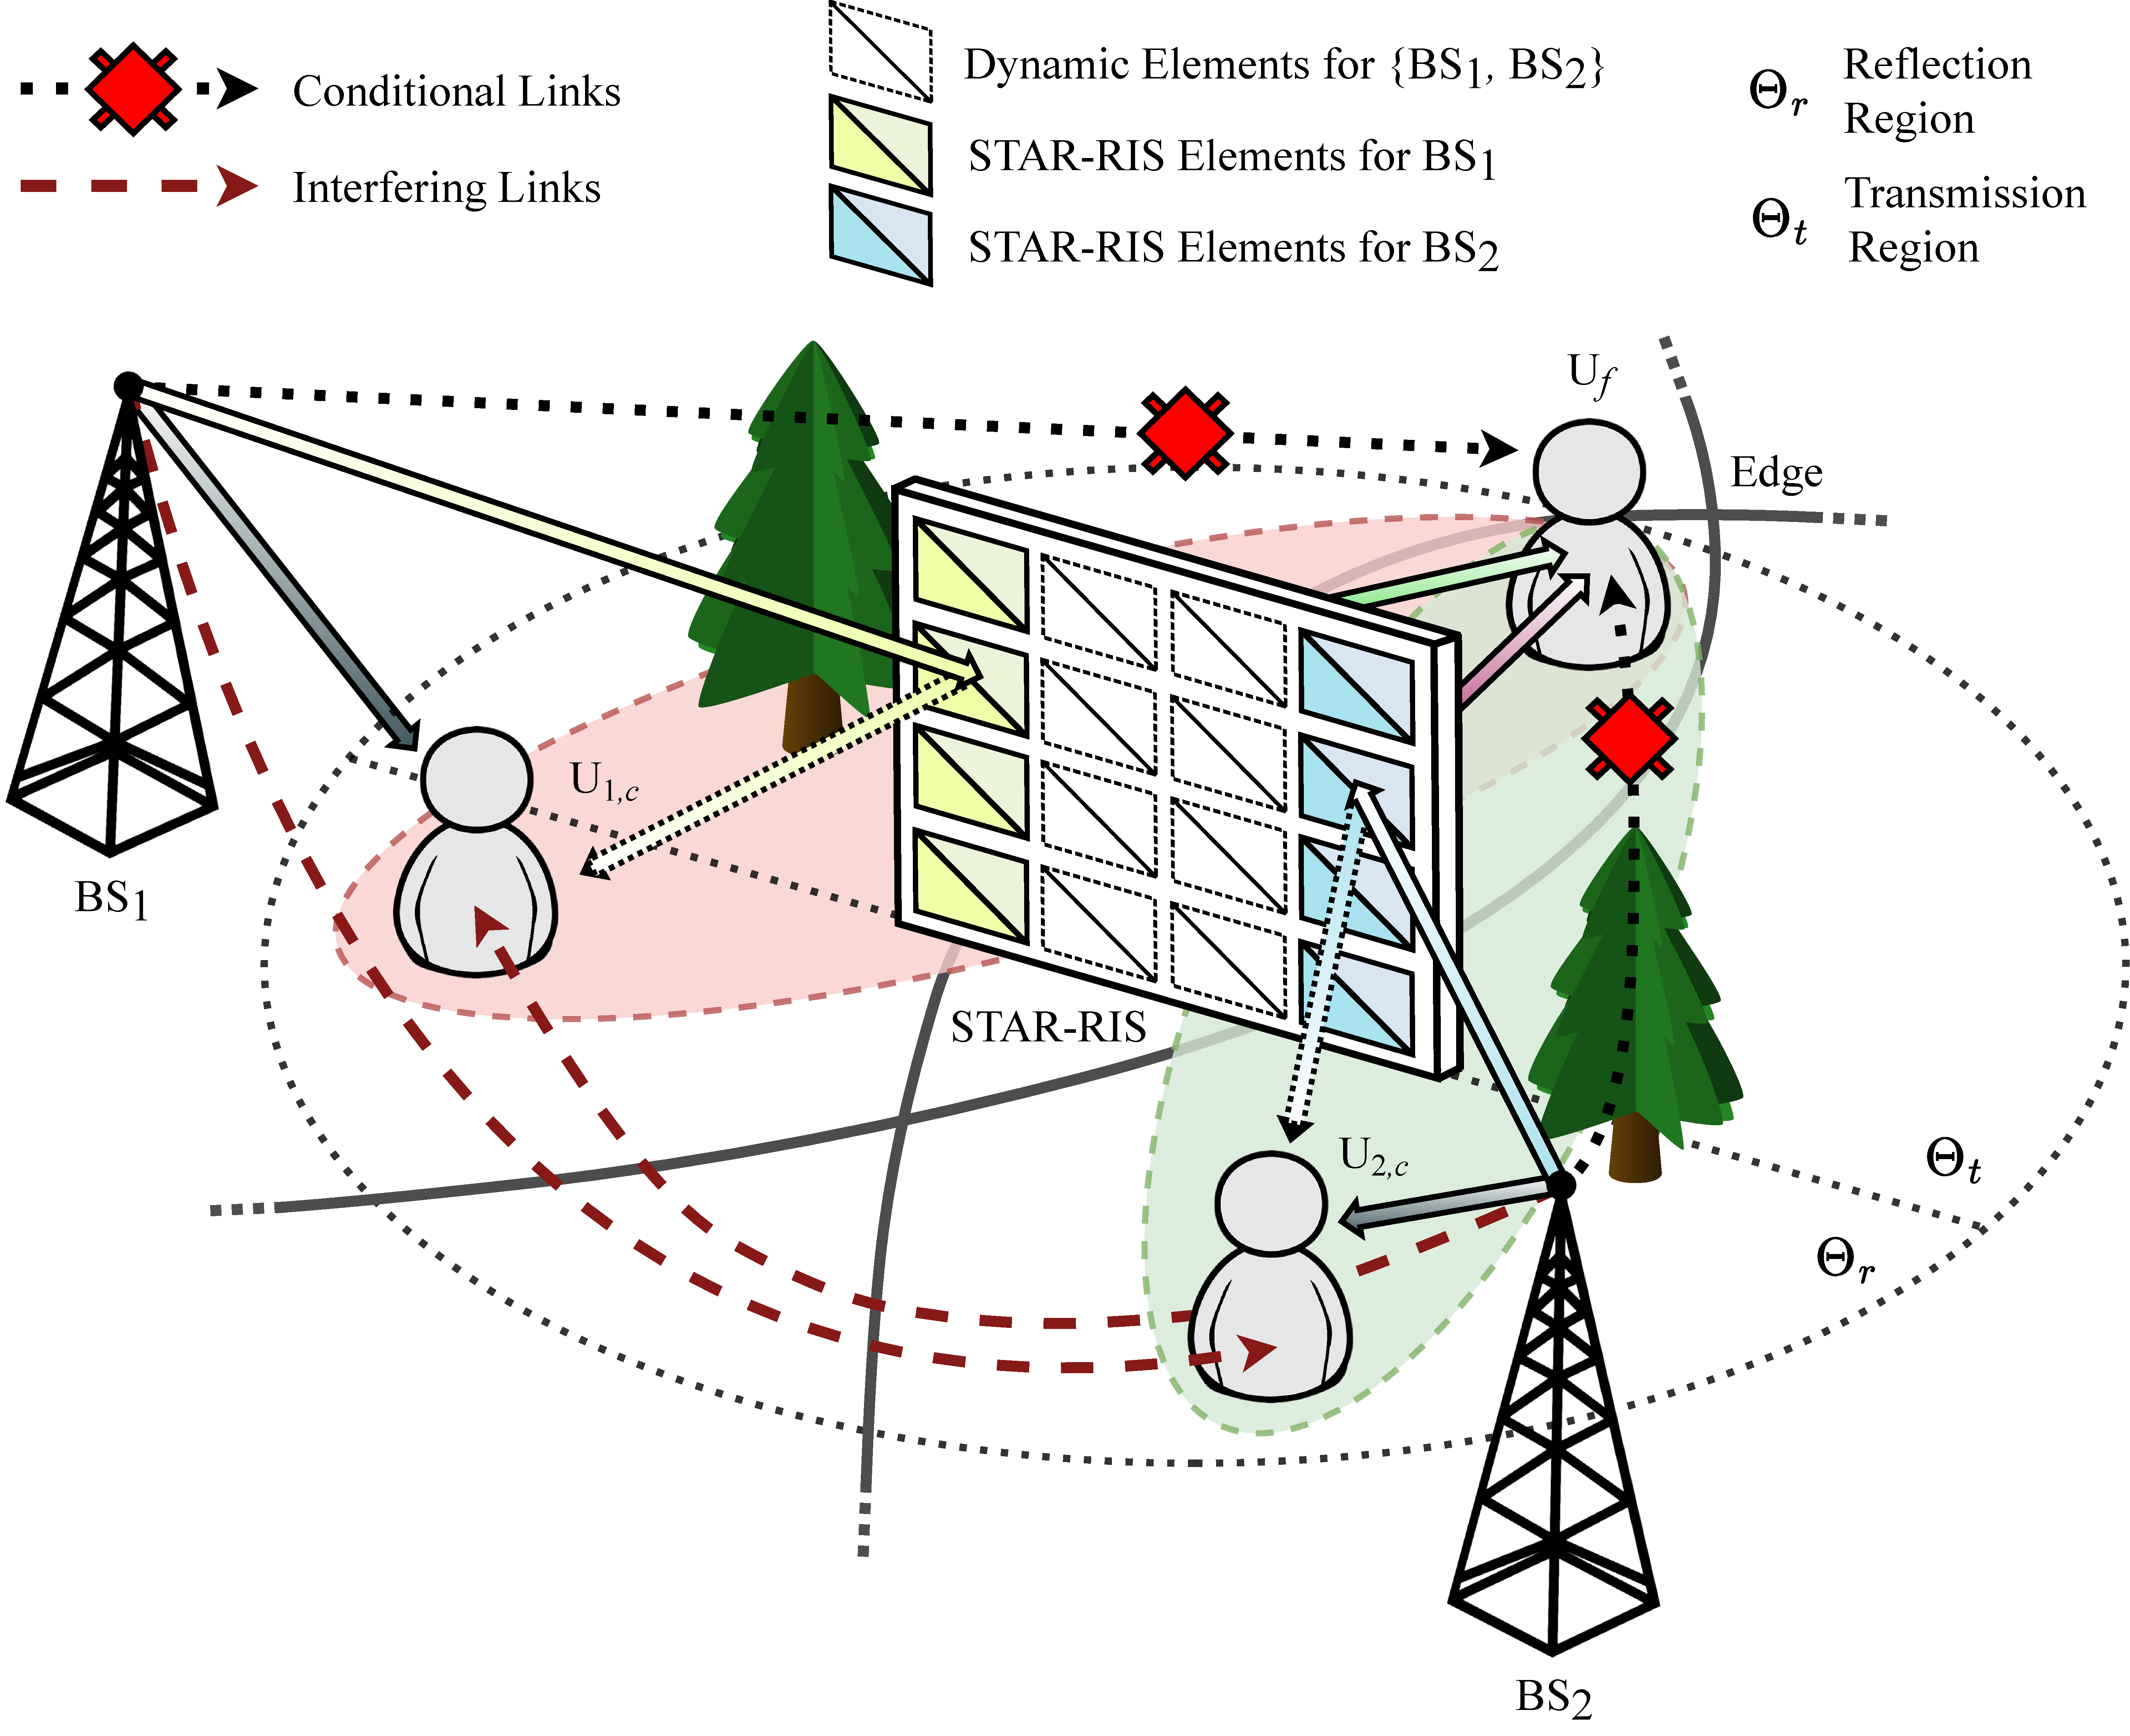
\includegraphics[width=0.45\textwidth]{figs/system.pdf}}
    \caption{An illustration of STAR-RIS-aided coordinated NOMA cluster.}
    \label{fig:system}
\end{figure}

The BSs employ power-domain NOMA techniques to communicate with the users. Specifically, $\forall i \in \mathcal{I}, c \in \mathcal{C}$, and $f \in \mathcal{F}$, BS$_i$ forms the NOMA pair (${\text{U}_{i,c}, \text{U}_f}$), where $\text{U}_{i,c}$ is the cell-center user of BS$_i$. Consequently, the U$_f$ is part of two NOMA pairs, each cluster served by a different base station. To mitigate the strong ICI experienced by U$_f$, CoMP is adopted between the two BSs. In addition, it is assumed that the BSs are connected to a central processing unit (CPU) via high-speed fronthaul links, facilitating seamless information sharing and coordinated transmissions among them.
% This particular user arrangement is defined as a coordinated NOMA cluster~\cite{elhattab2022ris}.
% Moreover, all users within the coverage region of $\text{BS}_1$ treat the signal received from $\text{BS}_1$ as the desired signal, while the signal received from the $\text{BS}_2$ is treated as interference. The same holds for users within the coverage region of $\text{BS}_2$. 

In this paper, perfect CSI is assumed to be available at the BSs. While this is a challenging assumption in practice, recent advances in channel estimation techniques for RIS-enabled wireless networks have shown that it is possible to achieve accurate CSI~\cite{hou2021joint, wei2021channel, taha2021enabling} with a reasonable amount of overhead. These estimation methods can also be applied to STAR-RISs, but are beyond the scope of this work.

\subsection{Channel Model}
For each communication link in the system, we take into account both large-scale fading and small-scale fading effects. Due to the relatively large propagation distances and the scattering effect of the links between B$_i$ and U$_u$, $\forall i \in \mathcal{I}$ and $u \in \mathcal{U}$, the channels are assumed to follow Rayleigh fading, expressed as:
\begin{equation}
    \textbf{h}_{i,u} = \sqrt{\frac{\rho_{o}}{PL(d_{i,u})}} \mathbf{v}_{i,u}
\end{equation}
where $\mathbf{v}_{i,u}$ is a complex Gaussian random variable that follows a Rayleigh distribution with zero mean and unit variance, $\rho_{o}$ is the reference path-loss at a distance of 1 m, $PL(d_{i,u})$ is the large scale path-loss, modeled as $PL(d_{i,u})=\left(d_{i,u}\right)^{\alpha_{i\rightarrow u}}$, where $d_{i, u}$ is the distance and $\alpha_{i\rightarrow u}$ is the path-loss exponent between the BS$_i$ and U$_u$, respectively.

On the contrary, the link between the STAR-RIS, denoted by $R$, and each Base Station BS$_i$ is assumed to exhibit a dominant line-of-sight (LoS) path~\cite{guo2020intelligent}. Therefore, these links are subject to the Rician fading, where their channel coefficients are expressed as 
\begin{multline}
	\textbf{h}_{i,R} = \\ 
	\sqrt{\frac{\rho_{o}}{PL(d_{i,R})}} \left( \sqrt{\frac{\kappa_{i,R}}{\kappa_{i,R} + 1}} \hat{\mathbf{v}_{i,R}} + \sqrt{\frac{1}{\kappa_{i,R} + 1}} \mathbf{v}_{i,R} \right),
\end{multline}
where $d_{i,R}$ is the distance between the BS$_i$ and $R$, $\kappa_{i,R}$ represents the Rician factor, $\hat{\mathbf{v}_{i,R}}$ represents the deterministic LoS components, and $\mathbf{v}_{i,R}$ denotes the complex Gaussian random variables, each following a Rayleigh distribution with zero mean and unit variance, thus representing the NLoS components. The links between $R$ and U$_u$, $\forall u \in \mathcal{U}$, are also modeled in a similar fashion.
\subsection{STAR-RIS Model}
The energy splitting (ES) model of the STAR-RIS array can be mathematically characterized by the following respective transmission- and reflection-coefficient matrices~\cite{mu2021simultaneously}:
\begin{align}
	\mathbf{\Theta_r} & = \sqrt{\beta^r}\text{diag}(e^{j \theta_1^t}, e^{j \theta_2^t}, \dots, e^{j \theta_K^t}), \\
	\mathbf{\Theta_t} & = \sqrt{\beta^t}\text{diag}(e^{j \theta_1^r}, e^{j \theta_2^r}, \dots, e^{j \theta_K^r}),
\end{align}
where $\beta^t$, $\beta^r \in [0, 1]$ and $\theta_k^t$, $\theta_k^r \in [0, 2 \pi)$, $\forall k \in \mathcal{K} \triangleq \{1, 2,\dots,K\}$. The phase shifts for transmission and reflection (i.e., $\theta_k^t$ and $\theta_k^r$) can generally be chosen independently of each other~\cite{9437234}. However, the amplitude adjustments for transmission and reflection are coupled by the law of conservation of energy. Assuming the STAR-RIS does not impose any power loss, the relation between the amplitude coefficients (i.e., $\beta^t$ and $\beta^r$) is expressed as $\beta^t + \beta^r = 1$. To reduce the signaling overhead between the STAR-RIS and the BSs, all elements are adjusted to have the same transmission and reflection coefficients.

% As the CSI is fully estimated at the BSs, the optimal phase shifts $\forall k \in \mathcal{K}$ can be computed as~\cite{wu2019intelligent}:
% \begin{equation}
%     \theta_k^p = \text{mod}[\arg(\textbf{h}_{i,q}) - \arg(\textbf{h}_{i,R}\cdot \textbf{h}_{R, q}),\,2\pi]
% \end{equation}
% where arg is the argument function and is utilized to compute the phase of the channels, $p \in \{t, r\}$ representing transmission and reflection regions of STAR-RIS, respectively, and $q \in \mathcal{C}$ when $p=t$, or $q \in \mathcal{F}$ when $p=r$.

\section{Performance Analysis}
\subsection{Rate Analysis}
To analyze the rates achieved for users in the system model shown in Fig. \ref{fig:system}, we first present the signal model. Specifically, $\forall i \in \mathcal{I}$, $c \in \mathcal{C}$, $f \in \mathcal{F}$, let the tuple (U$_{1,c}$, U$_{2,c}$, U$_f$) represent the coordinated NOMA cluster, and let $P_1$ and $P_2$ denote the transmit powers of BS$_1$ and BS$_2$, respectively. This signal model serves as the foundation for evaluating the achieved rates and optimizing the system performance in the considered cluster. Additionally, let $x_{1,c}$, $x_{2,c}$, and $x_f$ represent the message signal intended for U$_{1,c}$, U$_{2,c}$, and U$_f$, respectively. Each BS$_i$ broadcasts a superimposed signal of the messages~\cite{saito2013non} intended for users within its coverage region, U$_{i,c}$ and U$_f$, and expressed as:
\begin{equation}
    x_{i}=\sqrt{\zeta_{i,c}P_i}x_{i,c} + \sqrt{\zeta_{i,f}P_i}x_f,
\end{equation}
where $\zeta_{i,c}$ and $\zeta_{i,f}$ are the power allocation (PA) factors assigned by BS$i$ to users U$_{i,c}$ and U$_f$, respectively. It is important to note that U$_{i,c}$ experiences stronger channel conditions compared to U$_f$, making it the dominant NOMA user in the pair ($\text{U}_{i,c}, \text{U}_f$) formed by BS$i$. Following the principle of NOMA, U$_{i,c}$ should be capable of detecting and decoding the message intended for U$_f$. This principle also implies that $\zeta_{i,c} < 0.5$, or $0.5 < \zeta_{i,f} < 1$~\cite{obeed2020user, salem2020noma}.

For brevity, we only define the rate achieved by U$_{1,c}$ from the set of cell-center users $\mathcal{C}$, as the same steps could be extended to define the rate of U$_c$, $\forall c \in \mathcal{C}$. The received signal at U$_{i,c}$ can be written as:
\begin{equation}
    y_{1,c}=\textbf{h}_{1,c}x_1 + \textbf{h}_{2,c^\prime} x_2 + N_o,
\end{equation}
where $N_o$ is an additive white Gaussian noise (AWGN), i.e., $N_o\sim \mathcal{CN}$(0, $\sigma^2$). Further, $\textbf{h}_{2,c^\prime}$ is the channel corresponding to the link between BS$_2$ and U$_{1,c}$, which is the cell-center user of BS$_1$, and represents the ICI experienced at U$_{1,c}$. By utilizing successive interference cancellation (SIC) techniques, U$_{1,c}$ first decodes the message signal of U$_f$ (i.e., $x_f$) and then removes it from $y_{1,c}$ to decode its own message (i.e., $x_{1,c}$). Based on this approach, the achievable rate at U$_{1,c}$ for decoding the message of U$_f$ can be expressed as
\begin{equation}
    \mathcal{R}_{1,c\rightarrow f}=\log_2\left(1+\frac{\zeta_{1,f}P_1\abs{\textbf{H}_{1, c}}^2}{\zeta_{1,c}P_1\abs{\textbf{H}_{1, c}}^2 + P_2\abs{\textbf{h}_{2,c^\prime}}^2 +  \sigma^2}\right),
\end{equation}
where $\textbf{H}_{1, c}=\textbf{h}_{1, c}+\textbf{h}_{R, c}^H \mathbf{\Theta_r}\textbf{h}_{1, R}$ represents the combined channel from BS$_1$ to U$_{1,c}$. Furthermore, the achievable rate at U$_{1,c}$ for decoding its own message can be expressed as:
\begin{equation}
    \mathcal{R}_{1,c}=\log_2\left(1+\zeta_{1,c}\frac{P_1\abs{\textbf{H}_{1, c}}^2}{P_2\abs{\textbf{h}_{2,c^\prime}}^2 + \sigma^2}\right).
\end{equation}

On the contrary, U$_f$, belonging to two NOMA pairs, receives its signal through the broadcasts from each BS$_i$, $\forall i \in \mathcal{I}$. Thus, the received signal at U$_f$ can be expressed as
\begin{equation}
    y_f = \textbf{H}_{1, f}x_1 + \textbf{H}_{2, f}x_2 + N_0,
\end{equation}
where $\textbf{H}_{1, f}=\textbf{h}_{1, f}+\textbf{h}_{R, f}^H \mathbf{\Theta_t}\textbf{h}_{1, R}$ and $\textbf{H}_{2, f}=\textbf{h}_{2, f}+\textbf{h}_{R, f}^H \mathbf{\Theta_t}\textbf{h}_{2, R}$ denote the combined channels from BS$_1$ to U$_f$ and from BS$_2$ to U$_f$, respectively. As we considered non-coherent JT-CoMP, the achievable rate at U$_f$ can be expressed as~\cite{tanbourgi2014tractable, elhattab2022ris}:
\begin{equation}
    \mathcal{R}_{f}=\log_2\left(1 + \frac{\zeta_{1,f}P_1\abs{\textbf{H}_{1, f}}^2 + \zeta_{2,f}P_2\abs{\textbf{H}_{2, f}}^2}{\zeta_{2,c}P_1\abs{\textbf{H}_{1, f}}^2 + \zeta_{2,c}P_2\abs{\textbf{H}_{2, f}}^2 + \sigma^2}\right),
\end{equation}

% \begin{equation}
%     \mathcal{R}_{sum}=\sum_{i=1}^{2} \mathcal{R}_{i,c} + \mathcal{R}_{f}.
% \end{equation}

\subsection{Problem Formulation}
Based on the analysis conducted above, the joint network sum-rate optimization problem for a single coordinated NOMA cluster aided by the STAR-RIS can be formulated as
\begin{align}
\max_{\mathbf{\mathcal{A}}, \mathbf{\Theta}, \textbf{K}_A} \quad & \mathcal{R}_{\text{sum}}=\sum_{i=1}^{2} \mathcal{R}_{i,c} + \mathcal{R}_{f}, \label{eq:opt} \\
\textrm{s.t.} \quad & \mathcal{R}_f\geq\text{R}_\text{min}^f, \forall f \in \mathcal{F}, \nonumber \\
    \quad & \mathcal{R}_{i, c}\geq\text{R}_\text{min}^{i,c}, \forall i \in \mathcal{I}, c \in \mathcal{C}, \nonumber \\
    \quad & \zeta_{i,c}^2 + \zeta_f^2\leq1, \forall i \in \mathcal{I}, c \in \mathcal{C}, f \in \mathcal{F}, \nonumber \\
    \quad & \theta_k^t\in[0, 2\pi), k \in \mathcal{K} \nonumber \\
    \quad & \theta_k^r\in[0, 2\pi), k \in \mathcal{K} \nonumber \\
    \quad & \beta_t + \beta_r = 1, \nonumber \\
    \quad & P_i \leq \text{P}_\text{max}^i, i \in \mathcal{I}, \nonumber \\
    \quad & \sum_1^i \textbf{K}_A^i \leq K, i \in \mathcal{I}, k \in \mathcal{K}, \nonumber
\end{align}
where $\text{R}_\text{min}^f$ and $\text{R}_\text{min}^{i,c}$ represent the minimal achievable rates at U$_f$ and U$_{i,c}$, respectively. Further, $\text{P}_\text{min}^i$ is the maximum transmit power for each BS, whereas $\mathbf{\mathcal{A}}$ represents the PA factors of a single NOMA pair in the cluster. In addition, $\mathbf{\Theta}$ represents all the phase shifts associated with STAR-RIS, and $\textbf{K}_A$ is the splitting of STAR-RIS resources among the BSs.

As the CSI is fully estimated at the BSs, the optimal phase shift for each element $k \in \mathcal{K}$ can be computed~\cite{wu2019intelligent}, to solve the objective in \ref{eq:opt} as follows
\begin{equation}
    \theta_k^p = \text{mod}[\arg(\textbf{h}_{i,q}) - \arg(\textbf{h}_{i,R}\cdot \textbf{h}_{R, q}),\,2\pi],
\end{equation}
where $\arg(\cdot)$ is the argument function and is utilized to compute the phase of the channels, while $p \in \{t, r\}$ represents transmission and reflection regions of STAR-RIS, respectively. Also, $q \in \mathcal{C}$ when $p=t$, or $q \in \mathcal{F}$ when $p=r$. We adopt fixed empirical optimizations to address the joint network sum-rate optimization problem \ref{eq:opt}. Furthermore, we analyze the impact of distributing the STAR-RIS elements among the BSs by systematically exploring all conceivable splitting configurations through an exhaustive iteration process.

Advanced optimization techniques could potentially offer further improvements. However, the primary focus of this work is to showcase the fundamental enhancements attained by strategically deploying the STAR-RIS and distributing its resources among the Base Stations (BSs) within the coordinated NOMA cluster.

\section{Numerical Results}
This section presents numerical results for assessing the STAR-RIS enhancements in the proposed coordinated NOMA cluster.
\subsection{Simulation Setup}
We consider an outdoor environment where the transmission bandwidth of the network is set to $B = 1$ MHz, and the power of AWGN is set to $\sigma^2 = -174 + 10\log_{10}\left(B\right)$ (dBm) with a noise figure $N_F$ of $12$ dB. For simplicity, we assume that the transmit powers of both BS$_1$ and BS$_2$ are identical, expressed as $P_1 = P_2 = P_t$. Moreover, the PA factors for U$_{1,c}$, U$_{2,c}$, and U$_f$ are fixed to $\zeta_{1,c}=\zeta_{2,c}=0.3$ and $\zeta_f=0.7$, respectively.

In the three-dimensional Cartesian coordinate system, the locations of BS$_1$ and BS$_2$, each with a coverage radius of 60 m, are set to (-50m, 0m, 25m) and (50m, 0m, 25m) respectively. The STAR-RIS is strategically placed at the intersection of the two cells, near U$_f$, specifically, at the coordinates (0m, 25m, 5m). Additionally, the cellular users U$_{1,c}$, U$_{2,c}$, and U$_f$ are positioned at (-40m, 18m, 1m), (30m, 22m, 1m), and (0m, 35m, 1m), respectively. Some specific parameters used for simulation are outlined in Table \ref{tab:sim}.

\begin{table}[ht]
\centering
\setlength{\arrayrulewidth}{0.3pt} % Adjust the table border thickness
\caption{Simulation Parameters}
\resizebox{0.45\textwidth}{!}{\begin{tabular}{ll}
\hline
\textbf{Parameters} & \textbf{Values} \\ \hline \hline
Path-loss exponent of BS$_i$-U$_c$ links & $\alpha_{i\rightarrow c}=3$\\\hline
Path-loss exponent of BS$_i$-U$_f$ link & $\alpha_{i\rightarrow f}=3.5$\\\hline
Path-loss exponent BS$_i$-RIS links & $\alpha_{i\rightarrow R}=3$\\\hline
Path-loss exponent of RIS-U$_c$ links & $\alpha_{R\rightarrow c}=2.7$\\\hline
Path-loss exponent of RIS-U$_f$ link & $\alpha_{R\rightarrow f}=2.3$\\\hline
Path-loss exponent of Interfering links & $\alpha_{i\rightarrow c^\prime} = 4$\\\hline
Rician factor of RIS-U$_c$ links & $\kappa_{R\rightarrow c}=4$ dB\\\hline
Rician factor of RIS-U$_f$ link & $\kappa_{R\rightarrow f}=3$ dB\\ \hline
\end{tabular}}
\label{tab:sim}
\end{table}

\subsection{Impact of the Number of STAR-RIS Elements}
The outage probabilities and achievable rates for each user in the cluster are presented in Figs. \ref{fig:outage} and \ref{fig:rates}, respectively. With an increase in the number of elements $K$, we observe a notable reduction in outage probability of the cell-edge user U$_f$. This improvement is attributed to the enhanced data coverage facilitated by the STAR-RIS~\cite{wang2022outage}. Note that outage probabilities of U$_{1,c}$ and U$_{2,c}$ do not experience any substantial improvements, as their links are already dominated by the near base station BS$_1$ and BS$_2$, respectively. Moreover, due to strong ICI experienced by U$_f$ in the non-CoMP configuration, it experiences high outage probabilities, for all transmission power levels. The same trend is observed in the evaluation of user rates, with higher numbers of STAR-RIS elements leading to improved user rates.
\begin{figure}[t!]
    \centering
    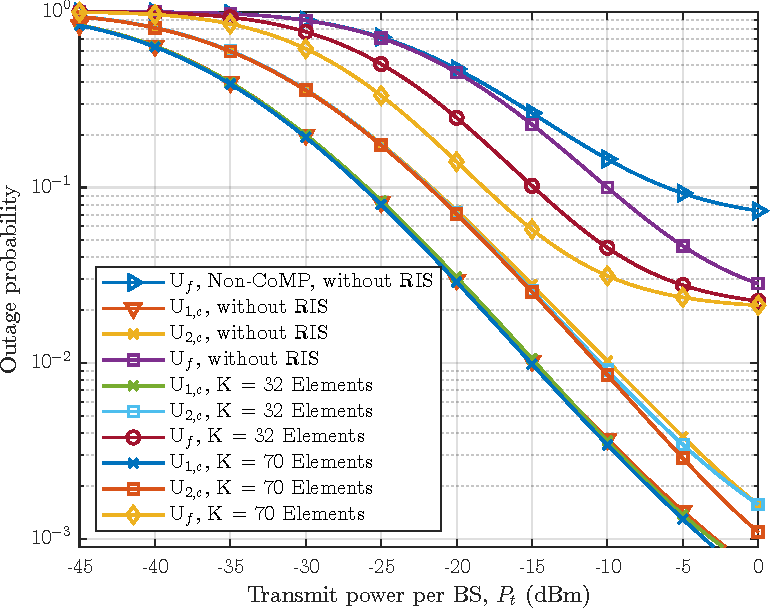
\includegraphics[width=0.45\textwidth]{figs/outage.pdf}
    \caption{Outage probability of all the users ($\text{U}_{1c}$, $\text{U}_{2c}$, $\text{U}_f$) versus $P_{t}$, for $\beta^t=0.5$, $\beta^r=0.5$, and $\textbf{K}_A^1=\textbf{K}_A^2=K/2$, when $K>0$.}
    \label{fig:outage}
\end{figure}
\begin{figure}[t!]
    \centering
    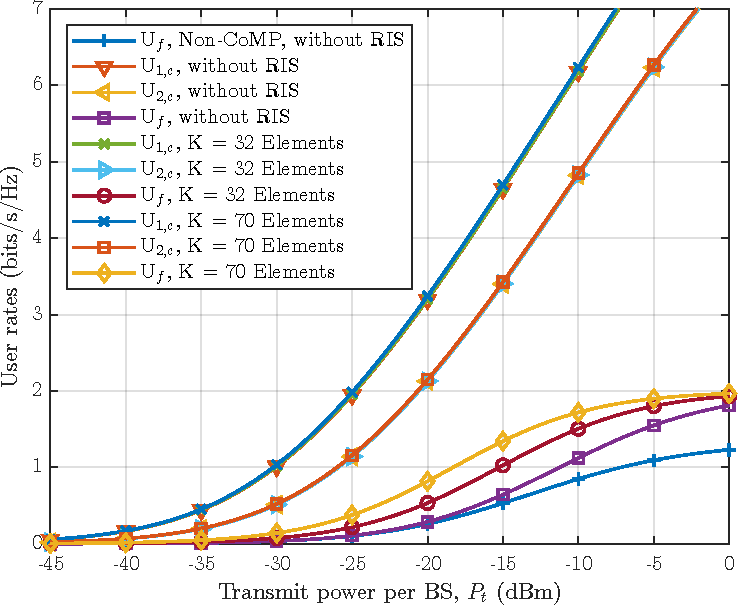
\includegraphics[width=0.45\textwidth]{figs/rates.pdf}
    \caption{Achievable rates of all the users ($\text{U}_{1c}$, $\text{U}_{2c}$, $\text{U}_f$) versus $P_{t}$, for $\beta^t=0.5$, $\beta^r=0.5$, and $\textbf{K}_A^1=\textbf{K}_A^2=K/2$, when $K>0$.}
    \label{fig:rates}
\end{figure}

\subsection{Coordinated NOMA Power Allocation Factors}
\begin{figure}[t!]
    \centering
    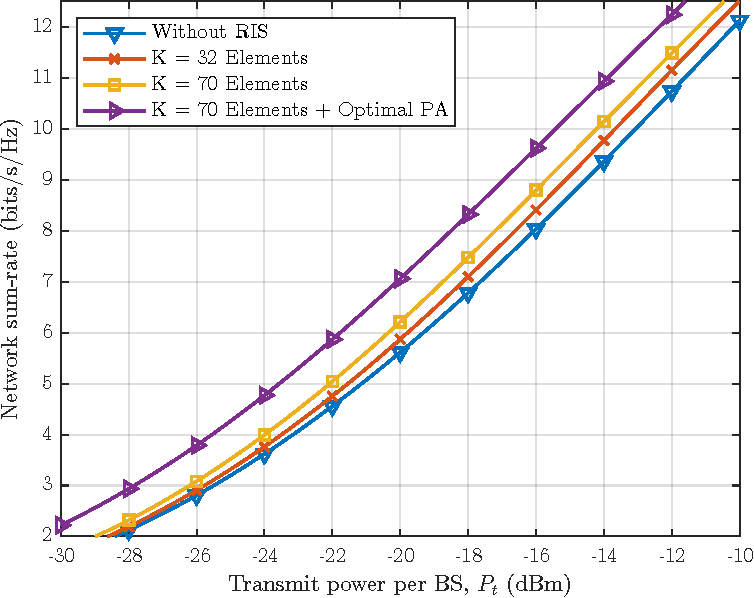
\includegraphics[width=0.45\textwidth]{figs/sumrate.pdf}
    \caption{Achievable network sum-rate versus $P_{t}$, for $\beta^t=0.5$, $\beta^r=0.5$, and $\textbf{K}_A^1=\textbf{K}_A^2=K/2$, when $K > 0$.}
    \label{fig:sumrate}
\end{figure}
The impact of PA factors in the coordinated NOMA cluster is evaluated in Fig. \ref{fig:sumrate}. The optimization problem of PA factors in a NOMA pair is formulated as follows
\begin{align}
\max_{\mathbf{\mathcal{A}}} \quad & \mathcal{R}_{i,c} + \mathcal{R}_{f}, \label{eq:opt2} \\
\textrm{s.t.}
    \quad & \zeta_{i,c}^2 + \zeta_f^2\leq1, \forall i \in \mathcal{I}, c \in \mathcal{C}, f \in \mathcal{F}, \nonumber
\end{align}
Following the methodology proposed in \cite{fang2016energy}, we obtain the optimal PA factors for the two NOMA pairs (i.e., ${\text{U}_{1,c}, \text{U}_f}$) and (${\text{U}_{2,c}, \text{U}_f}$). For the purpose of assessing the impact of power allocation factors on top of the STAR-RIS enhancements, we specifically focus on the case for a configuration with $K=70$ elements. Notably, this configuration yields the highest network sum-rate among all considered cases.

\subsection{Exhaustive STAR-RIS Element Allocation}
By performing exhaustive iterations over all potential combinations of STAR-RIS element assignments to BS$_1$ and BS$_2$ (i.e., $\textbf{K}_A^1=\textbf{K}_A^2=K/2$) in one dimension and exploring various transmission and reflection amplitude adjustments (i.e., $\beta_t$ and $\beta_r$) in another dimension, with $P_t = -15$ dBm, we plot the network sum-rate as a function of said dimensions. As evident from Fig. \ref{fig:dynamic}, the network sum-rate peaks when $\beta_t > \beta_r$. This observation aligns with the expectations, considering that the STAR-RIS is strategically positioned near U$_f$, located in the transmission region $\Theta_t$, thereby leading to an optimal network sum-rate.

\begin{figure}[t!]
    \centering
    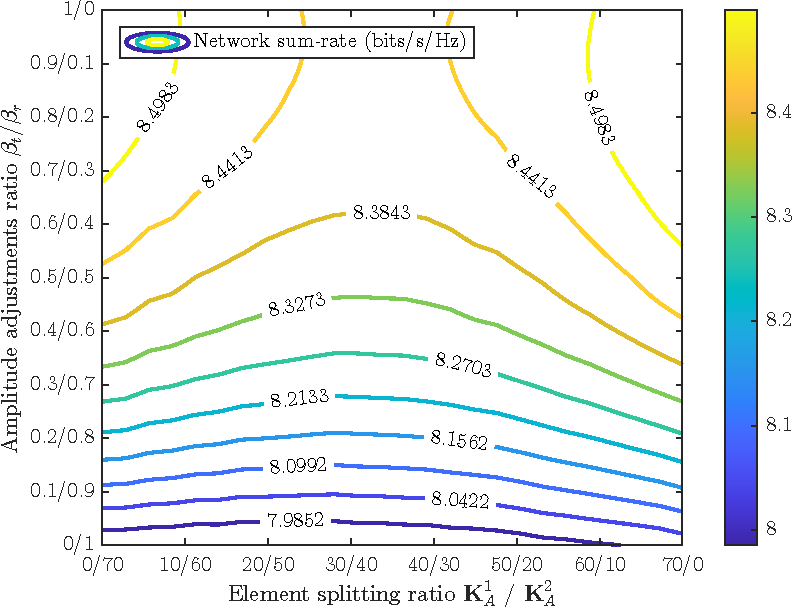
\includegraphics[width=0.47\textwidth]{figs/dynamic_s.pdf}
    \caption{Contour plot of network sum-rate as a function of STAR-RIS element allocation to BSs and amplitude adjustments ($\beta^t, \beta^r$) for $P_t =-15$ dBm.}
    \label{fig:dynamic}
\end{figure}

\subsection{Spectral Efficiency \& Energy Efficiency Trade-off}
In Figure \ref{fig:se_vs_ee}, we present the evaluation of the trade-off between spectral efficiency (SE) and electrical efficiency (EE). At circuit power $P_{\text{circuit}} = 1$ mW and the optimal operating point, it is evident that the CoMP-NOMA cluster assisted by STAR-RIS, with a larger number of elements $K$, achieves the highest EE. This observation can be attributed to the passive nature of STAR-RIS elements, which enhance the effective channel between the BSs and users by leveraging phase shifts, consequently resulting in a higher achievable network sum-rate.
\begin{figure}[t!]
    \centering
    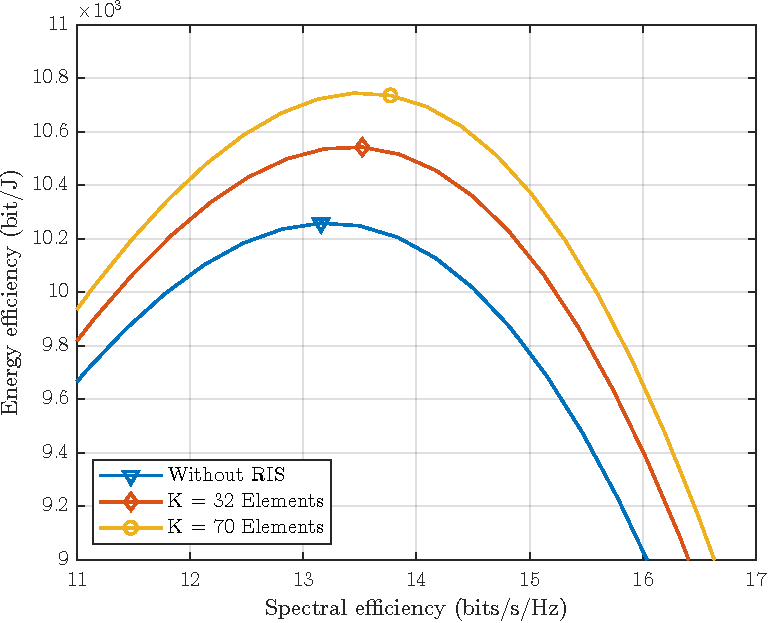
\includegraphics[width=0.45\textwidth]{figs/se_vs_ee.pdf}
    \caption{SE and EE trade-off with different STAR-RIS settings, for $P_{\text{circuit}} = 1$ mW, $P_t=-50:30$ dBm. Additionally, $\beta^t=0.5$, $\beta^r=0.5$, and $\textbf{K}_A^1=\textbf{K}_A^2=K/2$, when $K > 0$.}
    \label{fig:se_vs_ee}
\end{figure}

\section{Conclusion}
In this paper, we present a novel approach for STAR-RIS CoMP-NOMA networks, aiming to maximize data rates and improve outage conditions for all cellular users. By thoroughly optimizing STAR-RIS resources, this study effectively harnesses the synergies between STAR-RIS and CoMP-NOMA networks, resulting in elevated data rates and expanded data coverage. An essential aspect of our investigation is including the cell-edge user within NOMA pairs formed by each BS, leading to higher diversity gains. The outcomes of this study pave the way for potential future research directions, including exploring the proposed approach's scalability and adaptability to large-scale networks and diverse communication scenarios. Moreover, future extensions of this work include advanced optimization techniques, such as deep reinforcement learning, to address resource allocation challenges for future research endeavors.

\bibliographystyle{ieeetr}
\bibliography{references/ref}

\end{document}